%% PNAStwoS.tex
%% Sample file to use for PNAS articles prepared in LaTeX
%% For two column PNAS articles
%% Version1: Apr 15, 2008
%% Version2: Oct 04, 2013



%% BASIC CLASS FILE
\documentclass{pnastwo}




% And another fix.  PNAS class loses the label of floats unless they       
% were defined with the [h] option (so not really floats at all).  It      
% all comes down to wrong scope in the following routine which pushes      
% out the floats onto the page.  This is the fixed version:        
\makeatletter                                  
\def\DonormalEndcol{%                              
%% top float ==>                               
\ifx\toporbotfloat\xtopfloat%                          
%% figure ==>                                  
  \ifcaptypefig%                               
  \expandafter\gdef\csname topfloat\the\figandtabnumber\endcsname{%    
  \vbox{\vskip\PushOneColTopFig%                       
  \unvbox\csname figandtabbox\the\loopnum\endcsname%               
  \vskip\abovefigcaptionskip%                          
  \csname caption\the\loopnum\endcsname%                   
  \csname letteredcaption\the\loopnum\endcsname%               
  \csname continuedcaption\the\loopnum\endcsname%              
  \csname letteredcontcaption\the\loopnum\endcsname            
  \ifredefining%                               
  \csname label\the\loopnum\endcsname%                     
  \expandafter\gdef\csname topfloat\the\loopnum\endcsname{}\fi}%       
  \vskip\intextfloatskip%%                         
  \vskip-4pt %% probably an artifact of topskip??              
}%                                     
\else%                                     
%% plate ==>                                   
  \ifcaptypeplate%                             
  \expandafter\gdef\csname topfloat\the\figandtabnumber\endcsname{%    
  \vbox{\vskip\PushOneColTopFig%                       
  \unvbox\csname figandtabbox\the\loopnum\endcsname            
  \vskip\abovefigcaptionskip                           
  \csname caption\the\loopnum\endcsname                    
  \csname letteredcaption\the\loopnum\endcsname                
  \csname continuedcaption\the\loopnum\endcsname               
  \csname letteredcontcaption\the\loopnum\endcsname            
  \ifredefining                                
  \csname label\the\loopnum\endcsname                      
  \expandafter\gdef\csname topfloat\the\loopnum\endcsname{}\fi}        
  \vskip\intextfloatskip %%                            
  \vskip-4pt %% probably an artifact of topskip??              
}%                                     
\else% table ==>                               
 \expandafter\gdef\csname topfloat\the\figandtabnumber\endcsname{%     
 \vbox{\vskip\PushOneColTopTab %%                      
 \csname caption\the\loopnum\endcsname                     
  \csname letteredcaption\the\loopnum\endcsname                
  \csname continuedcaption\the\loopnum\endcsname               
  \csname letteredcontcaption\the\loopnum\endcsname            
  \vskip\captionskip                               
  \unvbox\csname figandtabbox\the\loopnum\endcsname            
\ifredefining                                  
\csname label\the\loopnum\endcsname                    
\expandafter\gdef\csname topfloat\the\loopnum\endcsname{}\fi           
}\vskip\intextfloatskip %% why don't we need this?             
\vskip-10pt}                                   
\fi\fi%                                    
%                                      
\else% bottom float                            
%                                      
\ifcaptypefig                                  
\expandafter\gdef\csname botfloat\the\figandtabnumber\endcsname{%      
\vskip\intextfloatskip                             
\vbox{\unvbox\csname figandtabbox\the\loopnum\endcsname            
\vskip\abovefigcaptionskip                         
  \csname caption\the\loopnum\endcsname                    
  \csname letteredcaption\the\loopnum\endcsname%               
  \csname continuedcaption\the\loopnum\endcsname%              
  \csname letteredcontcaption\the\loopnum\endcsname%               
\vskip\PushOneColBotFig%%                          
\ifredefining%                                 
\csname label\the\loopnum\endcsname                    
\expandafter\gdef\csname botfloat\the\loopnum\endcsname{}\fi}}%        
\else                                      
\ifcaptypeplate                                
\expandafter\gdef\csname botfloat\the\figandtabnumber\endcsname{%      
\vskip\intextfloatskip                             
\vbox{\unvbox\csname figandtabbox\the\loopnum\endcsname            
\vskip\abovefigcaptionskip                         
  \csname caption\the\loopnum\endcsname                    
  \csname letteredcaption\the\loopnum\endcsname%               
  \csname continuedcaption\the\loopnum\endcsname%              
  \csname letteredcontcaption\the\loopnum\endcsname%               
\vskip\PushOneColBotFig%%                          
\ifredefining%                                 
\csname label\the\loopnum\endcsname                    
\expandafter\gdef\csname botfloat\the\loopnum\endcsname{}\fi}}%        
  \else% TABLE                                 
\expandafter\gdef\csname botfloat\the\figandtabnumber\endcsname{%      
  \vskip\intextfloatskip                           
\vbox{\csname caption\the\loopnum\endcsname                
  \csname letteredcaption\the\loopnum\endcsname                
  \csname continuedcaption\the\loopnum\endcsname               
  \csname letteredcontcaption\the\loopnum\endcsname%               
  \vskip.5\intextfloatskip                         
  \unvbox\csname figandtabbox\the\loopnum\endcsname%               
\vskip\PushOneColBotTab                            
\ifredefining%                                 
\csname label\the\loopnum\endcsname                    
\expandafter\gdef\csname botfloat\the\loopnum\endcsname{}\fi}}%        
\fi\fi\fi}                                 
\makeatother  


%Fix wierd behavior which prevents table captions from appearing for
% tables in the body of the article
\makeatletter
\long\def\@makecaption#1#2{%
\ifx\@captype\table
\let\currtabcaption\relax
\gdef\currtabcaption{
\tabnumfont\relax #1. \tabtextfont\relax#2\par
\vskip\belowcaptionskip 
}
\else
 \vskip\abovecaptionskip
  \sbox\@tempboxa{\fignumfont#1.\figtextfont\hskip.5em\relax #2}%
  \ifdim \wd\@tempboxa >\hsize
\fignumfont\relax #1.\figtextfont\hskip.5em\relax#2\par
  \else
    \global \@minipagefalse
    \hb@xt@\hsize{\hfil\box\@tempboxa\hfil}%
  \fi
\fi
}
\makeatother

\setlength{\footskip}{.5in}
\usepackage{algorithm2e}
%% ADDITIONAL OPTIONAL STYLE FILES Font specification
\usepackage{natbib}
\usepackage{bm}% bold math
%\newcommand{\bm}[1]{\boldsymbol{#1}} %makes bold math symbols easier
\newcommand{\R}{\textsf{R}\space} %R in textsf font
\newcommand{\X}{\bm{\mathcal{X}}} %shorthand for iid
\renewcommand{\P}{\mathcal{P}}
\newcommand{\bt}{\pmb{\theta}}
\newcommand{\bl}{\pmb{\lambda}}
\newcommand{\bL}{\pmb{\Lambda}}
%\newcommand{\bG}{\pmb{\Gamma}}
\newcommand{\bh}{\pmb{\text{h}}}
\newcommand{\h}{\pmb{\text{h}}}
\usepackage{amsmath,amssymb,amsthm}
\def\citeapos#1{\citeauthor{#1}'s (\citeyear{#1})}
\DeclareMathOperator*{\argmax}{arg\,max}

%\graphicspath{{/Users/matthewjdenny/Dropbox/PINLab/Projects/Denny_Working_Directory/2011_Analysis_Output}}

%\usepackage{pnastwoF}
\usepackage{hyperref,booktabs,tabularx,float}


%% OPTIONAL MACRO DEFINITIONS
\def\s{\sigma}


\begin{document}

\title{Reading between the Emails: Gendered Patterns of Communication in Local Government}

\author{
Matthew Denny\affil{1}{Penn State University},
James ben-Aaron\affil{2}{University of Massachusetts Amherst},
Hanna Wallach\affil{2}{}\affil{3}{Microsoft Research NYC},
\and Bruce Desmarais\affil{1}{}
}

\contributor{\vspace{-.25cm}}


\maketitle

\begin{article}
\begin{abstract}
{We conduct an analysis of the relationship between gender and communication patterns in a sample of 17 North Carolina county governments. We apply an extension of the recently developed topic-partitioned multinetwork embeddings model to infer the content-conditional structure of manager-to-manager email communication in these county governments. We provide results which illustrate that while aggregate patterns of communication among department managers do not display significant gender bias, the content of communication and positions held by men and women differ significantly. We also find that some previously studied institutional-level factors seem to matter for the gendering of communication, and that women seem to be excluded from the locus of control in these organizations.
%We illustrate the use of covariates in the model with gender and find that patterns of gender mixing vary with the topical content of communication in a way that is consistent with the content-conditional gendered patterns that have been found to characterize social and organizational networks
}
\end{abstract} 

%\keywords{weighted networks |  | x-ray reflectivity | molecular electronics}

%\abbreviations{SAM, self-assembled monolayer; OTS, octadecyltrichlorosilane}

\section{Introduction}



% general overview of the solution we will develop and immediately related recent work
% Advances in statistical models for textual data \citep{Papadimitriou1998,Blei2003}
% have recently been built upon to

Researchers have recently begun to integrate structural models of networks with models for textual content \citep{McCallum2007,Krafft2012}. In this paper we introduce two extensions to the topic partitioned multi-network embeddings (TPME) model introduced by Krafft et al. \cite{Krafft2012}, and apply this model to the analysis of a large cross-organizational email corpus. Specifically, we extend the work of Krafft et al. to include actor-level covariates such as gender or organizational position, and latent-class topic clustering. These extensions situate our new model as a full generalization of the latent space network model \citep{Hoff2002a} to text-valued networks. Our approach allows us to discover varying content-conditional sub-structures within the email networks we study, that we are likely to miss when only examining the aggregate network structure (an example is provided in Figure \ref{fig:splitting}). 

We use our new model to understand how gender is related to the patterns of communication between department managers in 17 North Carolina county governments, and how these patterns vary with message content. This new dataset comprises almost 18,000 emails sent between 362 county department managers (e.g. health, budget, HR) during overlapping 3-month periods in 2013. Importantly, we were also able to gather covariate data for each manager, such as their gender and formal position in the organization, allowing us to make inferences about the relationship between these covariates and the observed network structure. Utilizing our model, we examine the variation in the propensity for men and women to send, and be included as recipients of emails, across content domains and counties. We find that while aggregate patterns of communication among department managers do not display significant gender bias, the content of communication and positions held by men and women differ significantly.


 \begin{figure}
\caption{\label{fig:splitting} Different patterns of communication across different domains.}	
\centering
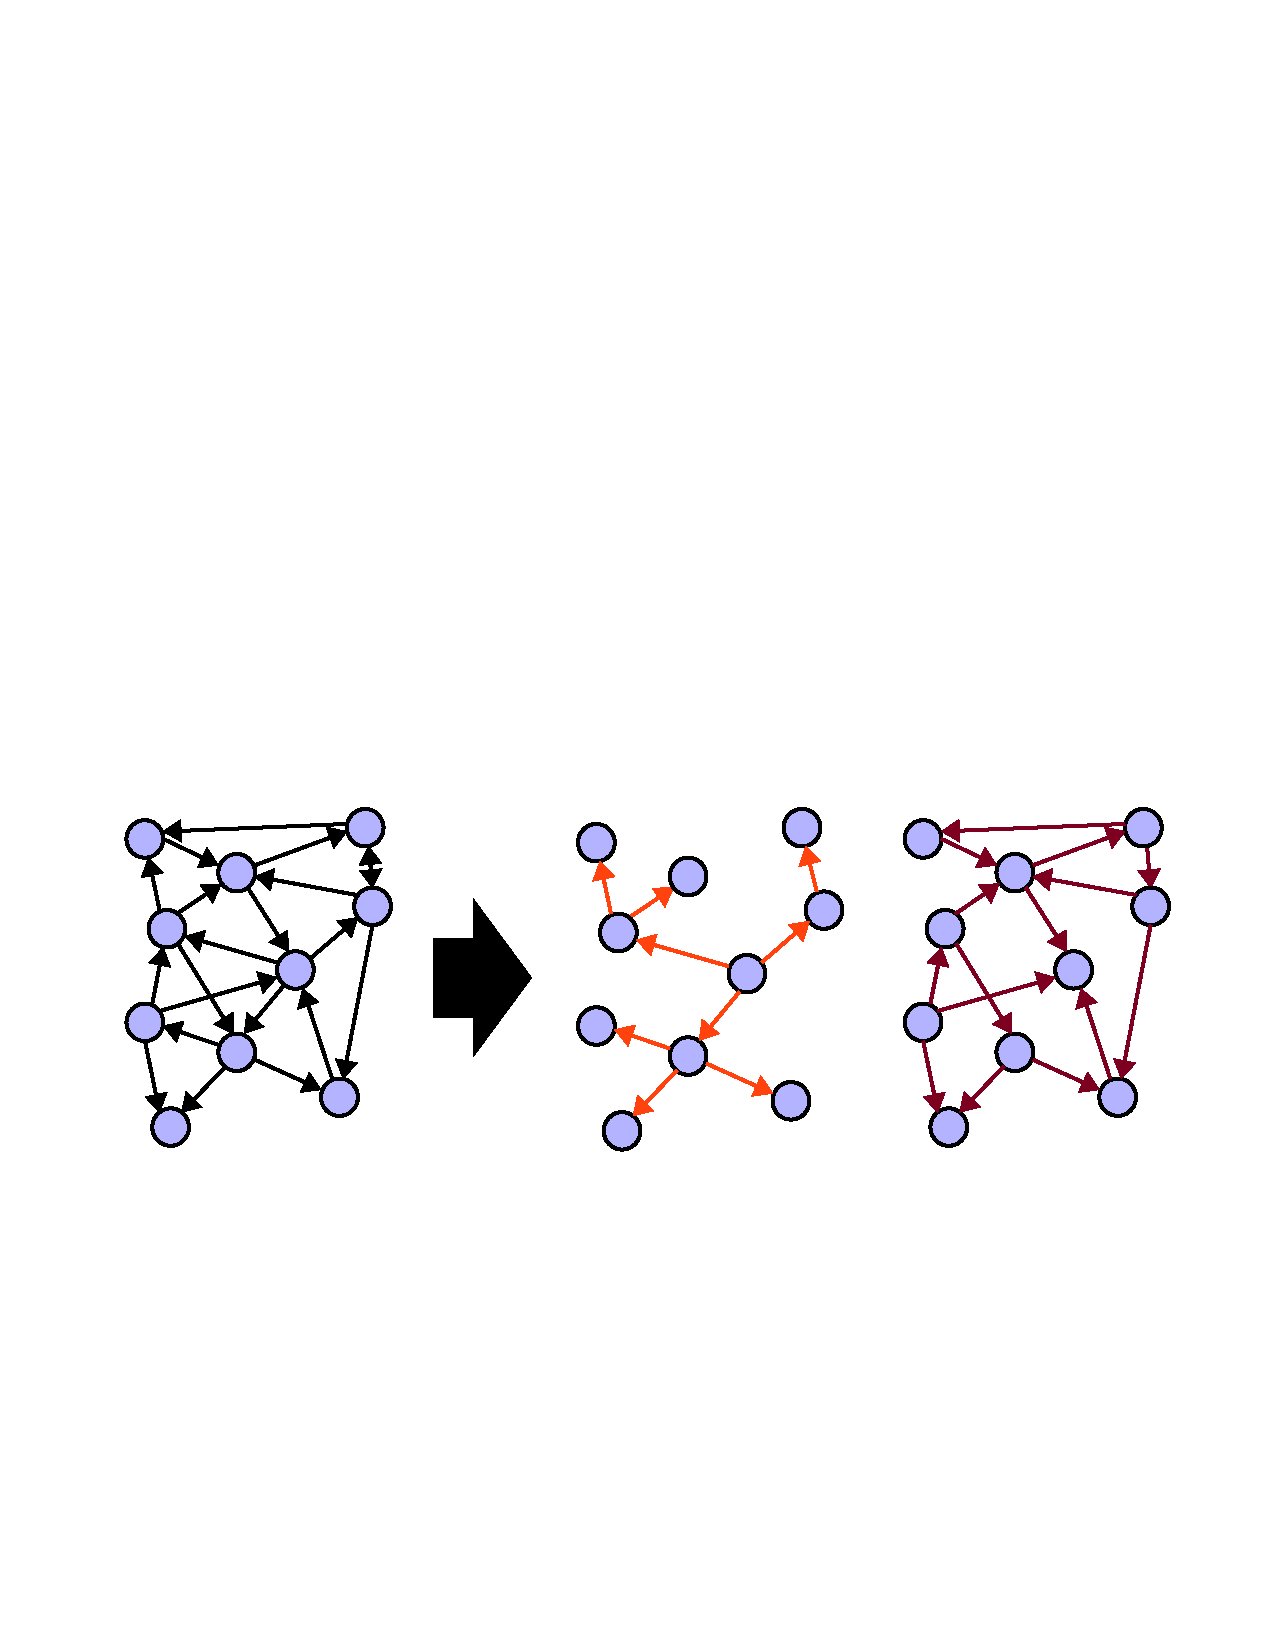
\includegraphics[width = 0.48\textwidth]{images/Structure_Matters_Full.pdf}
\end{figure}


\section{A Model for Communication Networks}
Here we provide a brief overview of our extension to the TPME model \citep{Krafft2012}. We focus on the ways in which our new model allows us to make inferences about the gender-specific patterns of communication in organizations, and how these patterns vary with the content of communication. Our model follows \citep{Krafft2012} by integrating the latent space network model \citep{Hoff2002a} with a statistical topic model (latent Dirichlet allocation \cite{Blei2003}) to jointly model the content and structure of a communication network. 

At a high level, our model assumes the following generative process for a message sent across the communication network. First, we sample the content of the message following the generative process for latent Dirichlet allocation. Then, for a given message sender, we sample whether each other actor in the network is a receiver of that message following the latent space network model. However, different topics (or clusters of topics in our extension) are associated with different latent spaces, so how likely each actor is to be a receiver of a particular message is dependent on the topical content of that message. We review this process in greater detail below.  

The message content is assumed to be generated via latent Dirichlet allocation. Under this model, we assume that all unique words in our vocabulary are associated to varying degrees with each of $T$ latent ``topics''. Each topic is then a distribution over unique words (or ``word types''), $\boldsymbol{\phi}^{(t)}$. For example ``doctor'', ``virus'', and ``medicine'' might all have high probability in a topic about hospitals, while ``cat'' and ``music'' might have low probability in that topic. We further assume that each topic distribution is drawn from a Dirichlet prior: 
\begin{equation}
	\boldsymbol{\phi}^{(t)} \sim \text{Dirichlet}(\beta,\boldsymbol{n}) \text{ for } t = \{1, ..., T\}
\end{equation}
The concentration parameter $\beta$ controls how peaky this distribution is (how few word types will have high probability in a given topic), and the base measure $\boldsymbol{n}$ controls the bias in the degree to which word types will be assigned high probability in topics generally. For example, ``patient'' might generally have a higher probability than most word types in a corpus of documents about healthcare.   

To generate each of the $D$ documents (messages) in our corpus, we first draw a document-specific distribution over topics
\begin{equation}
	\boldsymbol{\theta}^{(d)} \sim \text{Dirichlet}(\alpha,\boldsymbol{m}) \text{ for } d = \{1,...,D\}
\end{equation}
Here, the concentration parameter $\alpha$ controls how topically specific the documents generated are, and $\boldsymbol{m}$ controls the bias in how likely certain topics are to appear. Once we have sampled our document-specific distribution over topics we can then generate each of $N$ tokens (words) in the document via a two step process. First we draw the latent topic assignment for that token from the document specific distribution over topics.
\begin{equation}
	z_n^{(d)} \sim \boldsymbol{\theta}^{(d)} \text{ for } n = \{1,...,N\}
\end{equation}
 Then we draw the word type of that token from the topic specific distribution over word types.
 \begin{equation}
 	w_n^{(d)} \sim \boldsymbol{\phi}^{(z_n^{(d)})} \text{ for } n = \{1,...,N\}
 \end{equation}
We proceed in this manner for all tokens in all documents. 

% The content of each message sent across the network is assumed to be generated similarly to the generative process for latent Dirichlet allocation, where each message is a mixture of different ``topics'', but the mixture of topics, and thus words, is governed in part by the (intended) recipients of that message.  The sender then selects the recipients for that message probabilistically, based on the message content and the associated content-specific latent social structure of the network.

In our extension of TPME, we further assume each topic is uniquely associated with one of $C$ clusters, sampled from a discrete uniform distribution.
\begin{equation}
	C_t \sim \text{Discrete Uniform}(1,C) \text{ for } t = \{1, ..., T\}
\end{equation}
The intuition is that different broad content areas of communication (e.g. ``planning'', ``sports'',``meeting planning'') -- each of which is a collection of more specific topics -- will imply a different pattern of communication. Importantly, under this model, a message can be about a number of topics, and these topics can be associated with different clusters. Each cluster is associated with a different pattern of communication, so the receivers for any particular message must be sampled following an add-mixture of several underlying communication patterns. For example, if a department manager in an organization sent an email message to schedule a budget meeting, they would likely include both staff whose job includes setting up meetings, and staff who needed to provide input on the budget as recipients. 

Finally, for a given cluster $c$, the probability that an actor is selected as a recipient of a particular message is specified by the latent space network model \citep{Hoff2002a}. Under this model, we assume there is some baseline propensity to include message recipients on any email, which is governed by an intercept parameter.
\begin{equation}
	b^{c} \sim \text{Normal}(\mu, \tau^2)
\end{equation} 
For example, messages about sensitive HR matters will probably include fewer recipients than messages announcing a department party. Second, some attributes of the sender and potential receiver (which we assume are observed) may also affect the probability of that actor being a recipient. The effect that each of these $L$ different attributes have on the probability of an actor being included as a message recipient can then be parameterized by a vector: 
\begin{equation}
	\mathbf{\gamma}_l^{c} \sim \text{M. V. Normal}(\mathbf{\lambda}, \mathbf{\eta}^2) \text{ for } l = \{1, ..., L\}
\end{equation}
For example, there is a great deal of social science literature showing that people tend to preferentially communicate with others of the same gender. Our model could generate this propensity by sampling positive parameters for Male-Male and Female-Female communication, and negative parameters for Female-Male and Male-Female communication. 

The additional variation (not captured by covariate effects) in the probability that a message is sent between two actors is governed by how close they are in a $k$ dimensional ``latent social space''. This latent space captures all un-modeled factors associated with the propensity for two actors to form a tie. In a typical social network this might include difficult or impossible to measure quantities like how nice a person is, or whether two people have ``chemistry''. Additionally, it may capture observable traits that the researcher was unable to collect data on (e.g. sexual orientation, or ethnicity). This makes the latent positions difficult to interpret when including covariates in the model, so great care should be taken when doing so. To capture these latent positions, each actor $a$ is assumed to have some position in the $k$-dimensional latent space
\begin{equation}
	\mathbf{s}_a^{c} \sim \text{M. V. Normal}(0, \sigma^2) \text{ for } a = \{1, ...,A\}
\end{equation}
and the probability that they send a message to an actor $r \neq a$ is decreasing in their latent distance from $r$. Thus the probability of actor $r$ being a recipient of a message from actor $a$ under this model is:
\begin{equation}
	P(y_{a,r}^{c} = 1) = \text{logit}^{-1}\left( b^c + \sum_L \left[\mathbf{X}_{a,r}^{l} \mathbf{\gamma}_l^{c}\right] - |\mathbf{s}_a^{c} - \mathbf{s}_r^{c}| \right)
\end{equation}
where $\mathbf{X}^{l}$ is a matrix recording the type of an edge for attribute $l$ that would be sent between $a$ and $r$ (e.g. Male to Female or employee to supervisor). Edge values for an individual message are then sampled via Bernoulli trials. However, the probability that $y_{a,r} = 1$ for a given message $d$ may be dependent on multiple latent spaces (because documents can be about multiple topics). The weight given to $P(y_{a,r}^{(c)})$ for each cluster is determined by the proportion of tokens in the message that are assigned to topics associated with cluster $c$.  
\begin{equation}
	P(y_{a,r}^{(d)} = 1) = \sum_C P(y_{a,r}^{c} = 1) \times *
\end{equation}
where $*$ is the proportion of tokens in document $d$ assigned to topics associated with cluster $c$.

Given that we do not directly observe the generative process, the object of inference becomes the posterior distribution of our model parameters given the data. This problem is analytically intractable, so we must approximate the posterior distribution via Markov chain Monte Carlo methods. We perform inference for this model via block Metropolis within Gibbs sampling\footnote{The inference algorithm is currently implemented in a beta version as an R package, and is available here: \href{https://github.com/matthewjdenny/ContentStructure}{github.com/matthewjdenny/ContentStructure}}. A further discussion of this model will be provided in a related paper, but this model provides a powerful and flexible framework to investigate the content-conditional gendered patterns of communication in an organization. 

\section{Data}
To better understand how gender is related to patterns of communication within government bureaucratic organizations, we examine overlapping three-month samples of email messages sent between department managers in 17 North Carolina county governments. The data used in this study were collected in 2013 via a series of FOIA requests, as part of a transparency-by-conformity field experiment involving all 100 North Carolina county governments. We received approximately 500,000 total emails from the 17 participating county governments, of which approximately 120,000 were classified as not spam after an intensive data cleaning and validation process\footnote{A technical report detailing the email cleaning  and preprocessing procedure is available upon request.}. Figure \ref{fig:nc map} highlights those counties which did respond to our requests for data\footnote{These counties are statistically indistinguishable from the general population of counties in North Carolina on a number of demographic dimensions.}.

We also collected detailed metadata on the position and gender of the 362 department managers in our sample. We display some basic descriptive statistics for each county in Table \ref{tab:county aggregate stats}. Table \ref{tab:email agg stats} reports some additional manager-to-manager email communication statistics by gender. These statistics are aggregated across all departments in all counties. Note that emails may have multiple recipients and thus we distinguish between the number of unique emails sent and the number or proportion of recipients. 

\begin{figure}
\caption{\label{fig:nc map} North Carolina county map.}	
\centering

\includegraphics[width = 0.48\textwidth]{images/County_Map.pdf}
\end{figure}



\begin{table}
	
	\begin{tabular}{lrrrrr}
	  \hline
	 \textbf{County} & \textbf{Mgrs.} & \textbf{Female} & \textbf{Internal} &\textbf{Total} \\
	  \hline
	Alexander & 21 & 9 & 907 & 11,924  \\
	Caldwell & 20 & 8 & 121 &    \\
	Chowan & 23 & 11 & 2,027 & 11,737  \\
	Columbus & 24 & 10 & 920 & 12,707  \\
	Dare & 27 & 12 & 2,247 &   \\
	Duplin & 27 & 14 & 1,914 &   \\
	Hoke & 24 & 11 & 1,106 & 5,565  \\
	Jackson & 24 & 6 & 1,499 &   \\
	Lenoir & 20 & 5 & 560 & 10,499 \\
	Lincoln & 22 & 7 & 573 & 8,727  \\
	McDowell & 17 & 5 & 326 & 3,494  \\
	Montgomery & 18 & 10 & 680 & 2,465  \\
	Nash & 19 & 8 & 1,147 & 9,133 \\
	Person & 21 & 9 & 1,491 & 14023  \\
	Transylvania & 20 & 4 & 1,857 & 14,088 \\
	Vance & 18 & 8 & 185 & 4,349  \\
	Wilkes & 17 & 2 & 303 & 8,443  \\
	   \hline
	   \textbf{Totals:} & 362 & 139 & 17,863 & 117,154  \\
	   \hline
	\end{tabular}
	\caption{\label{tab:county aggregate stats}Participating county email statistics. \textbf{Mgrs.} is the total number of department managers in a county, \textbf{Female} is the number of female managers in that county, \textbf{Internal} is the number of emails sent between managers in a county, and \textbf{Total} is the total number of emails sent and received by department managers in each county in our sample. Note that in this study, we only make use of the internal email data. Some email \textbf{Total}'s are omitted due to challenges in determining which emails (not sent by managers) were valid in these counties.}
\end{table}	
	

\begin{table}
	
	\begin{tabular}{m{2in}rrr}
	\toprule
& \textbf{Male} & \textbf{Female}  \\
	 \midrule
	 Proportion of All Managers in Sample & 61.6\%& 38.4\% \\

	 Total Emails Sent & 10,771 & 7,092 \\
	 Average Emails Received Per Manager & 70.8 & 71.6 \\
	 Average Number of Recipients Per Email Sent & 1.45 & 1.43 \\

	 Proportion of Emails Recipients of Same Gender & 60.7\% & 37.8\%  \\

	 Proportion of Emails Sent to County Manager & 24.4\% & 17.9\%  \\
	\bottomrule
	\end{tabular}
	\caption{\label{tab:email agg stats}Email statistics by gender.}
\end{table}


\section{Analysis} 
% The large figure above illustrates preliminary model results for the largest topic clusters in two North Carolina governments. Each model was run for 2,000 iterations with 1,000 iterations of Metropolis Hastings for each iteration of Gibbs sampling. Models were initialized with 50 topics and 10 clusters, but tend to select for 2-4 clusters with any topics assigned to them, indicating a lower dimensional space of communication patterns. To generate estimates of LSM positions, we run the last iteration of the LSM portion of the model until Geweke statistics demonstrate convergence on greater than 90\% of all parameters (5M iterations). Our results indicate that men tend to dominate the locus of control within these organizations, but that this pattern is uneven across counties, and dependent on organizational positions occupied by women.

% \begin{figure}
% 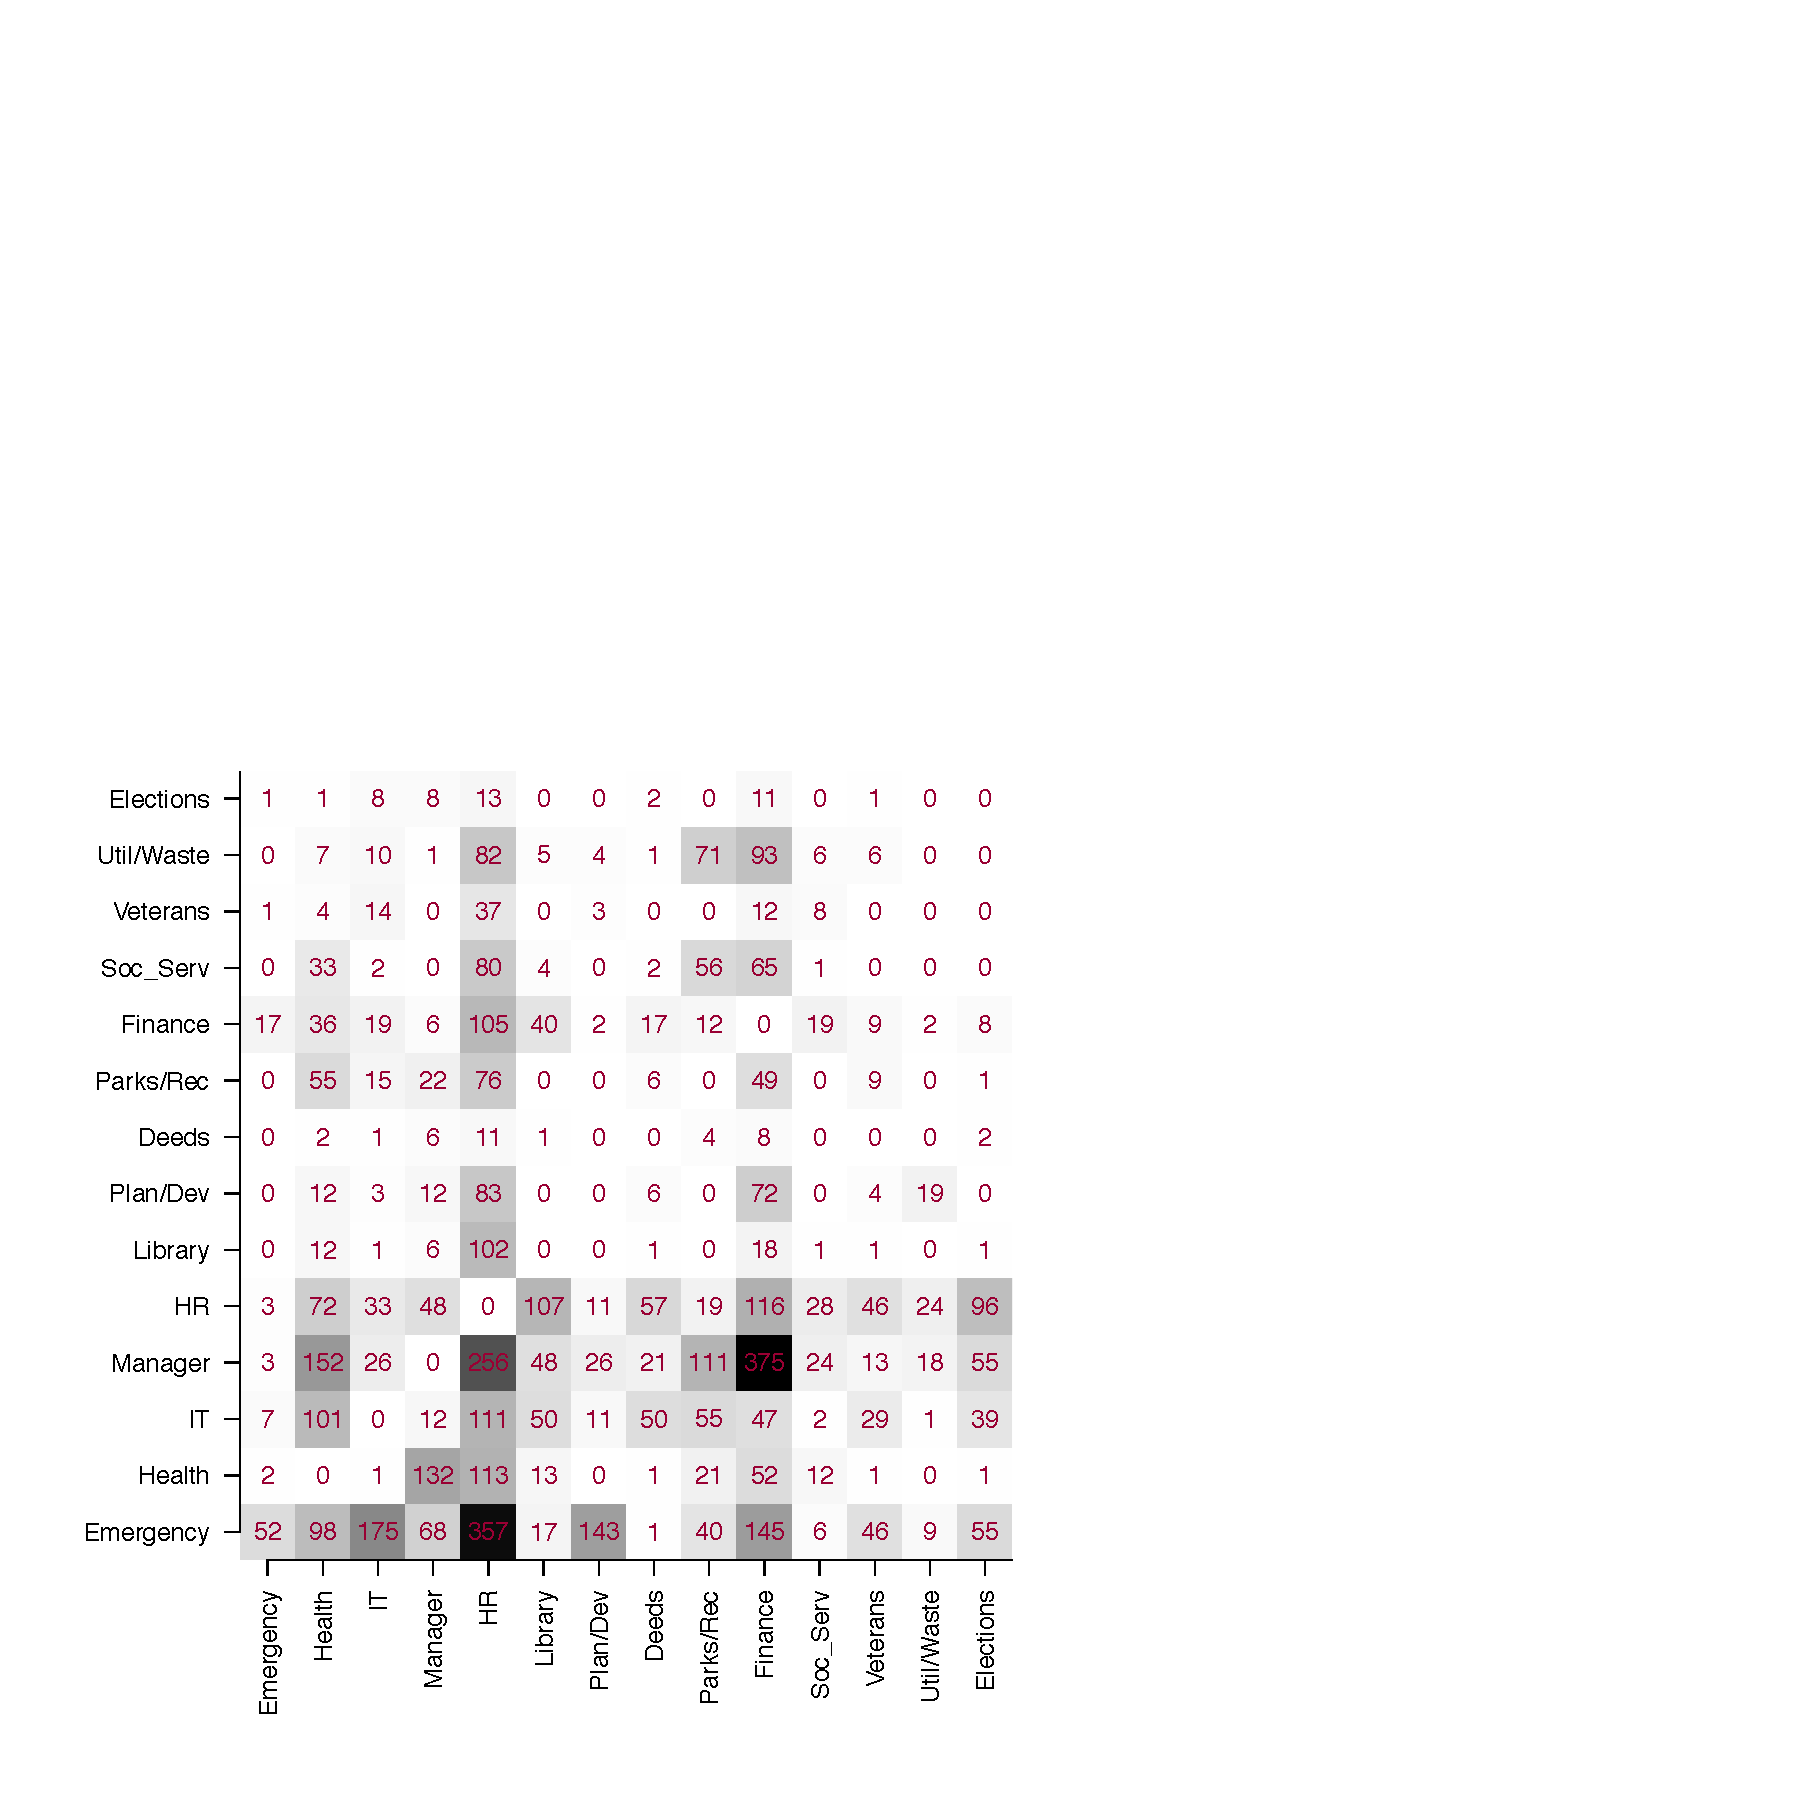
\includegraphics[width = 0.42\textwidth]{images/Female_Received_Flows.pdf}
% \caption{\label{fig:female heat}Prop. Emails Received by Female Dept. Managers}
% \end{figure}k


To begin understanding the relationship between gender and the patterns of communication within these county governments, we can look at the descriptive statistics in Table \ref{tab:email agg stats}. We see that women make up 38\% of managers in our sample and they send and receive 39-40\% of emails. Importantly, in aggregate, neither men nor women show a strong preference for within gender communication. Therefore, if a preference for same-gender communication exists within these organizations, aggregate level statistics do not capture it. However, these basic descriptive statistics ignore both the formal positions of email senders and recipients, and the email content. 

To delve deeper into these patterns of communication, we present four heat maps in Figure \ref{fig:heatmaps}. These heat maps record the number of emails sent to, and received by department managers given that they were male (female). As we can see, there are significant differences in the number of emails received by male and female managers working in the same department. Most striking is the almost complete absence of emails sent by the county manager to female department managers, whereas male department managers receive the largest proportion of their incoming emails from the county manager. For example, while male finance managers received approximately 40\% of their emails (485) from the county manager across all counties in our sample, female finance managers only received 6 emails from the county manager across our entire sample. This differential could reflect gender homophily in communication, given that 15 out of the 17 county managers in our sample are male. However, it may also be linked to the consistent finding in the gender-in-organizations literature that women are excluded from the ``locus of control'' in organizations. 



\begin{figure*}
\centering
\begin{tabular}{cc}
\textbf{Messages sent by male department managers} & \textbf{Messages received by male department managers}\\
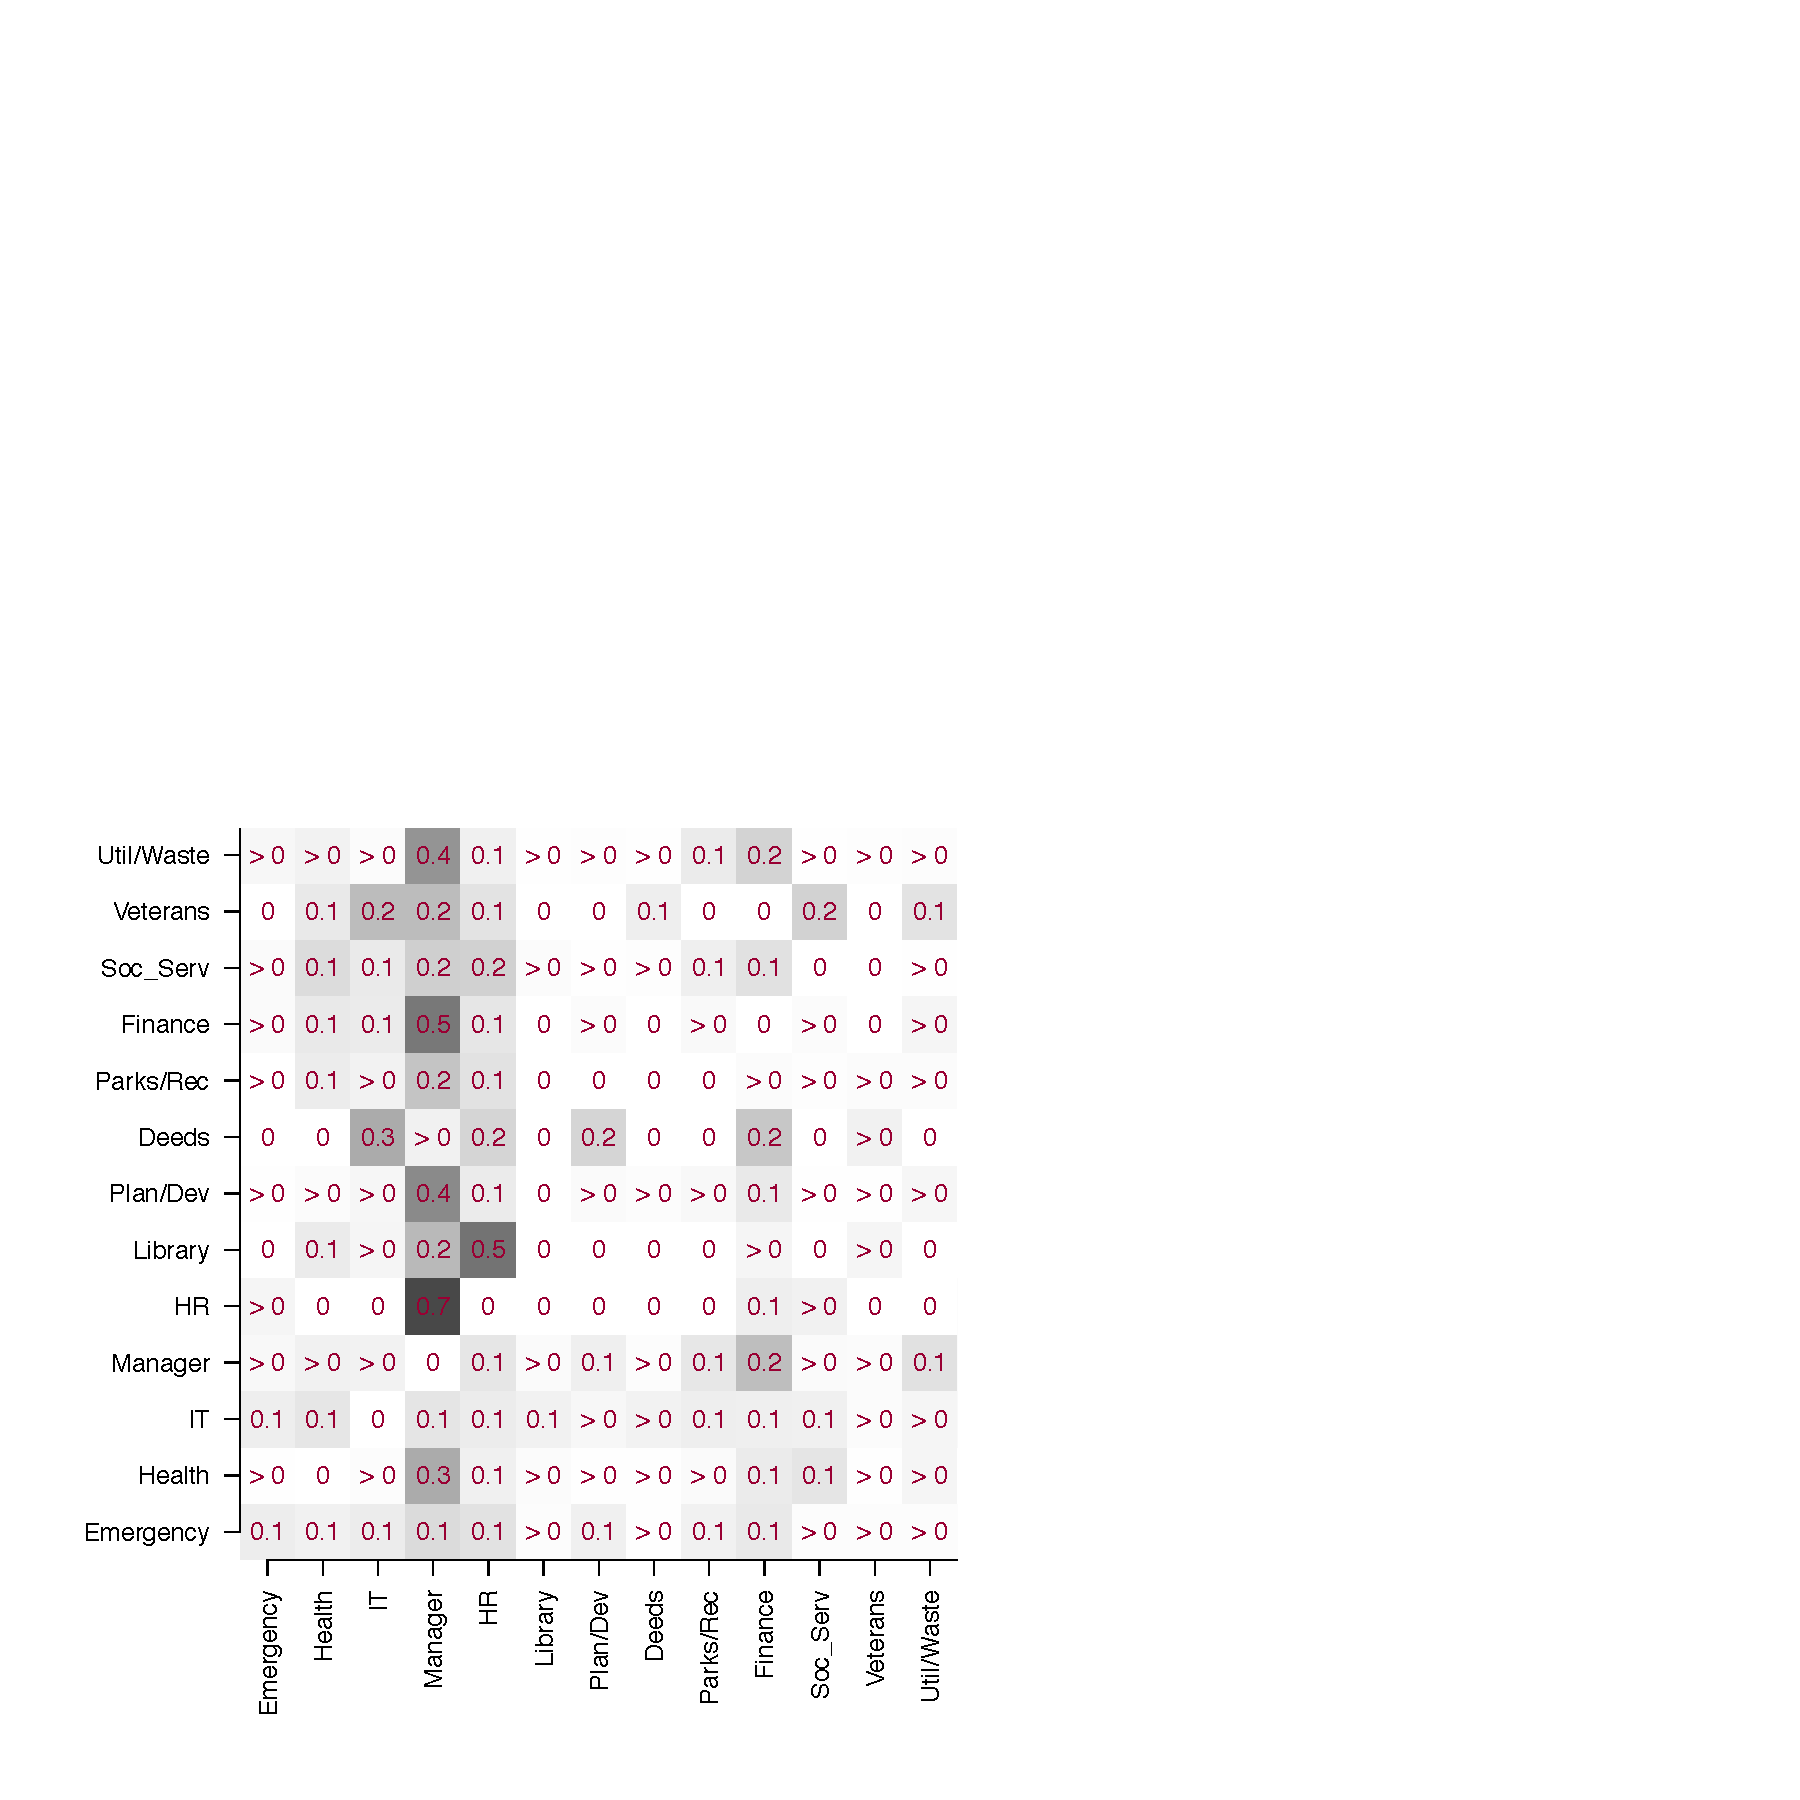
\includegraphics[width = 0.49\textwidth]{images/Male_Sent_Prop.pdf} &
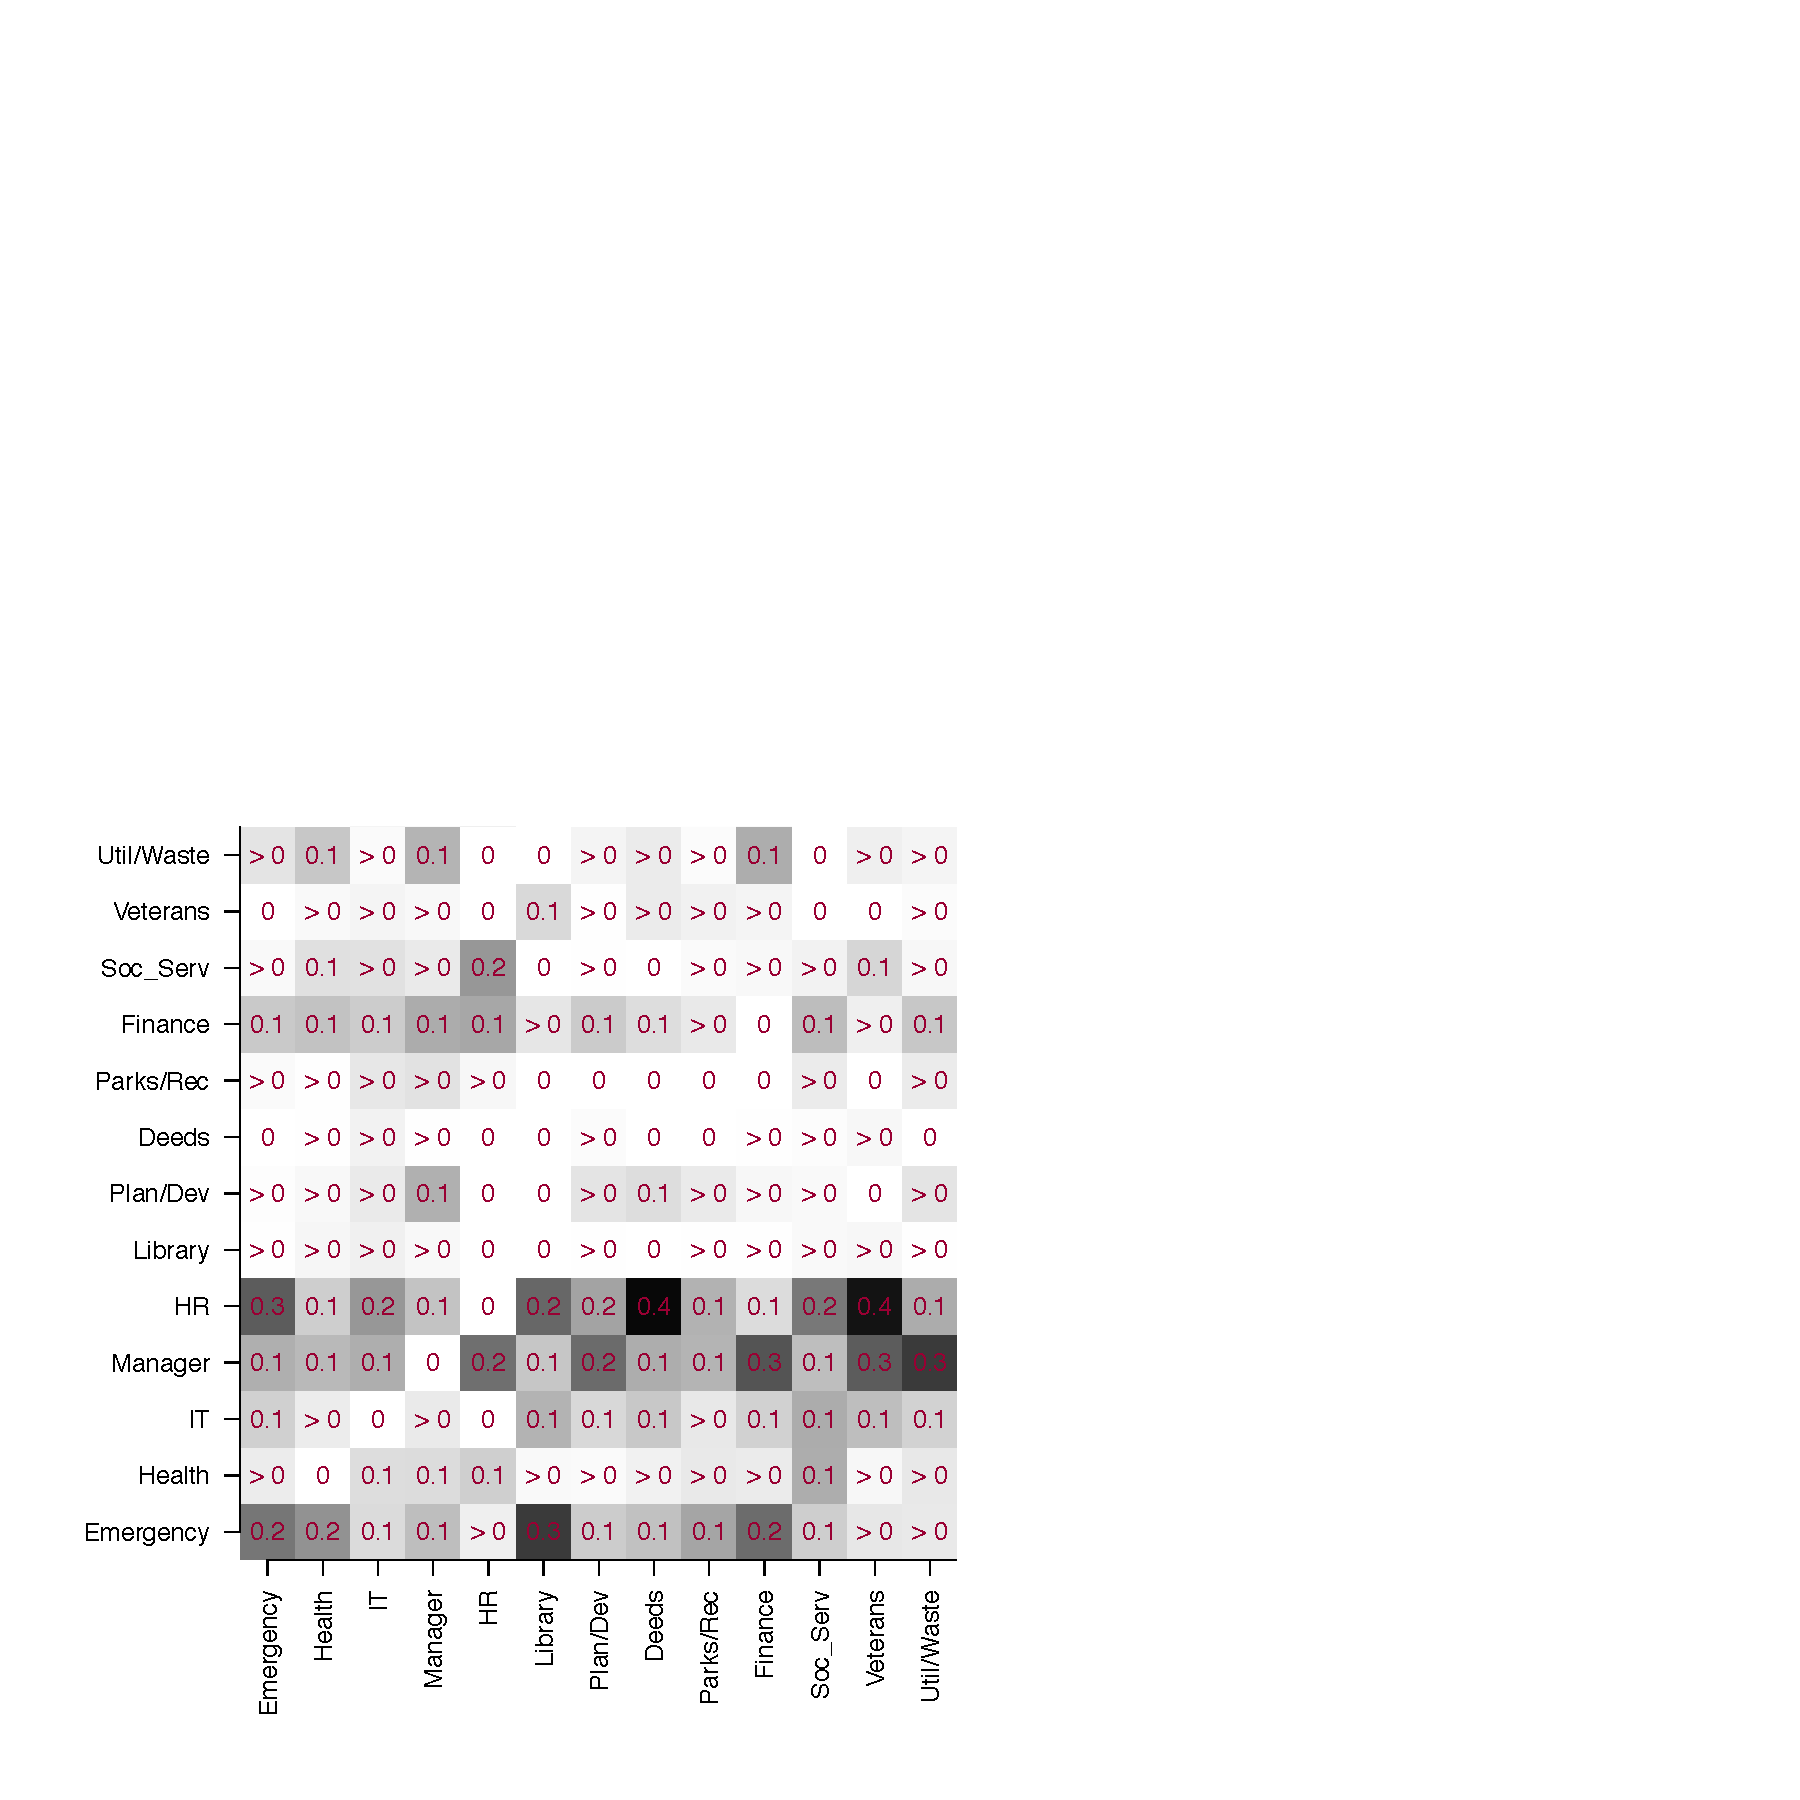
\includegraphics[width = 0.49\textwidth]{images/Male_Received_Prop.pdf} \\
\textbf{Messages sent by female department managers} & \textbf{Messages received by female department managers}\\
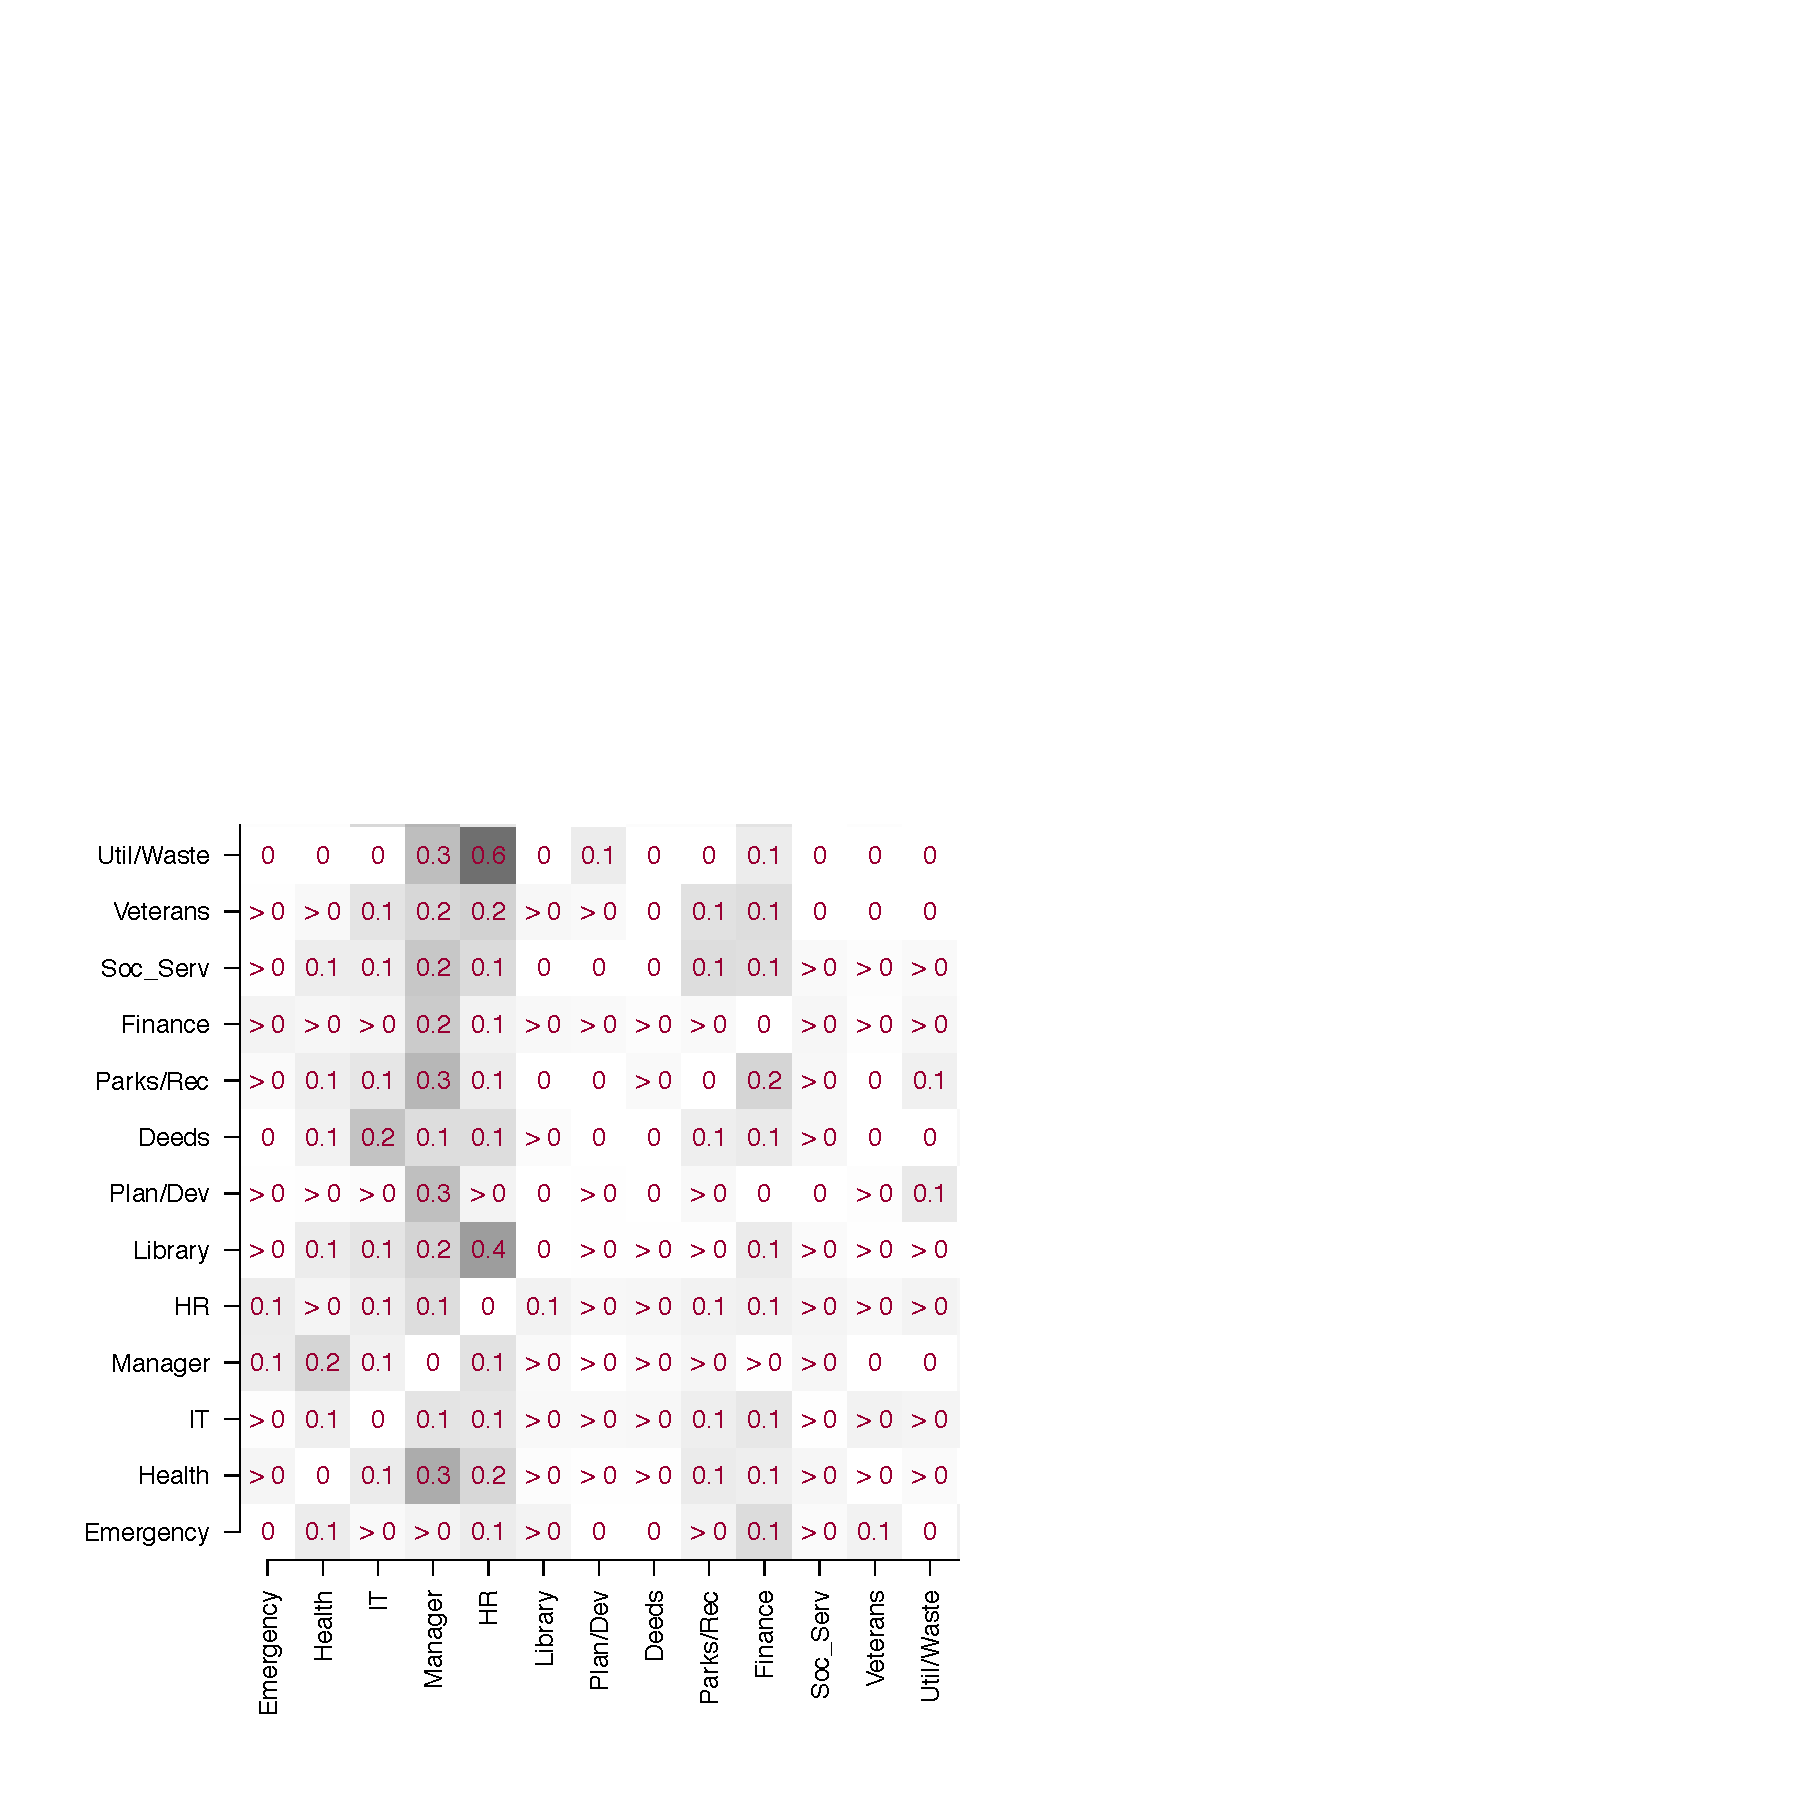
\includegraphics[width = 0.49\textwidth]{images/Female_Sent_Prop.pdf} &
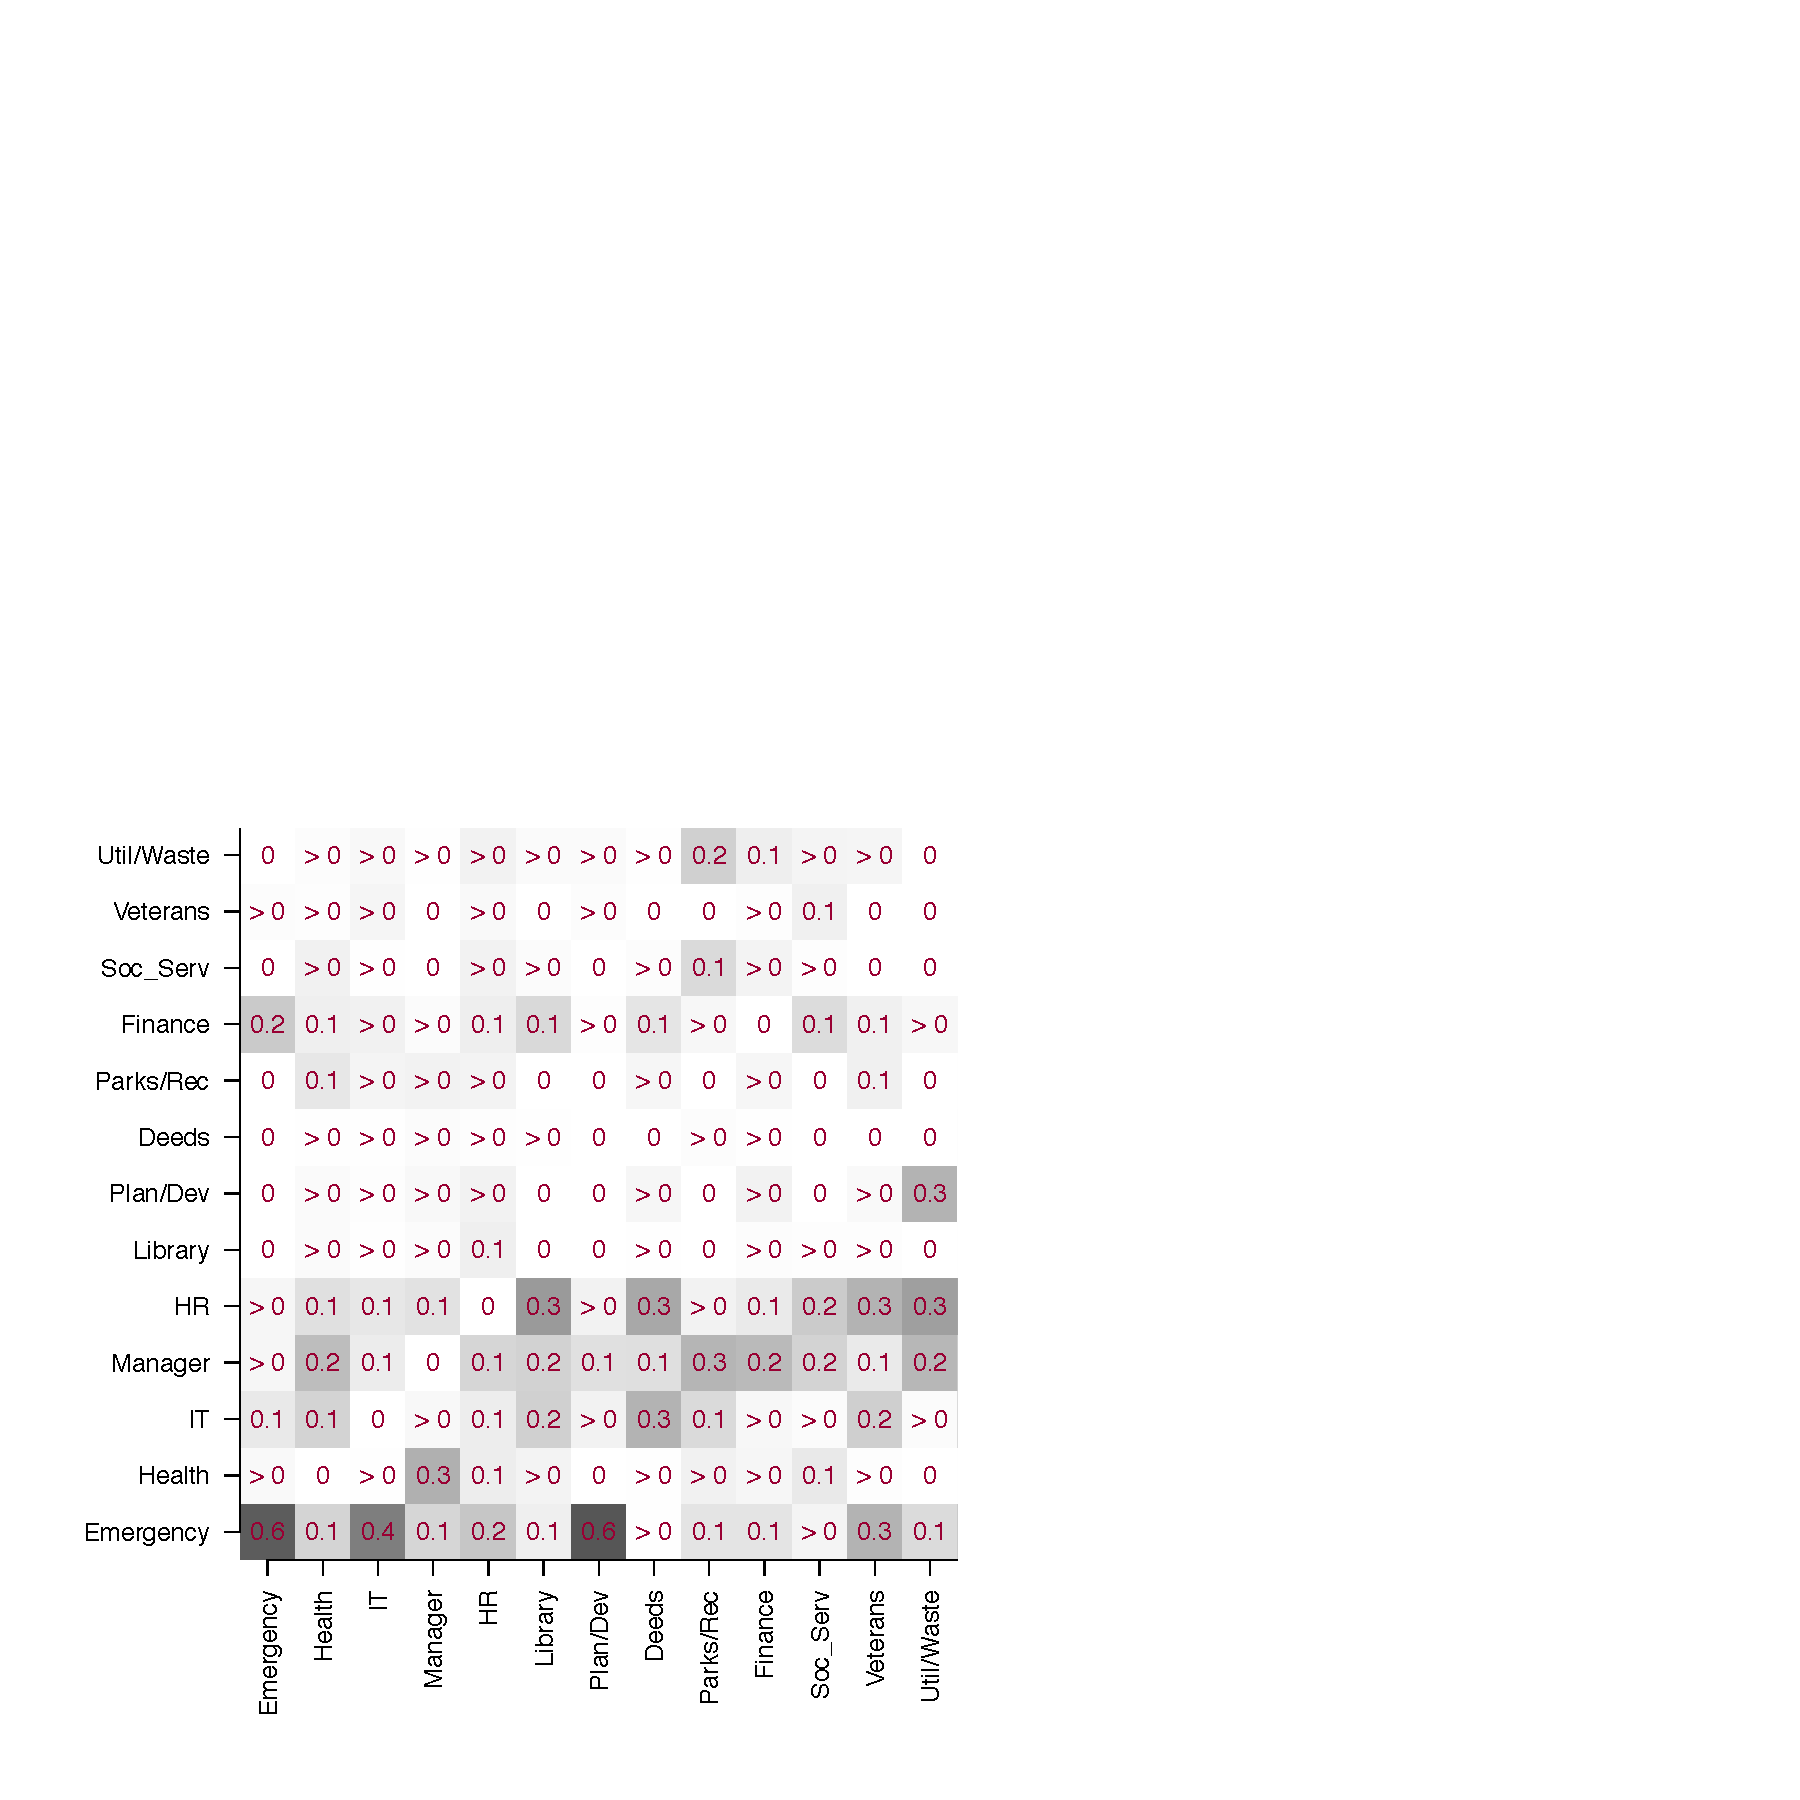
\includegraphics[width = 0.49\textwidth]{images/Female_Received_Prop.pdf}
\end{tabular}
\caption{\label{fig:heatmaps}Heat maps depicting the number of emails sent from the row department to the column department aggregated across counties and by gender. Departments were also hand coded into one of 25 different categories based on given titles to group departments that perform a similar function. The smallest 11 departments by email volume are omitted from these tables for readability but they display a similar pattern of communication.}
\end{figure*}
	
\subsection{Model-Based Inference}
Our initial analysis of the aggregate patterns of interaction in these organizations indicates that there are likely differences in the way department managers in the same organizational position communicate, by gender. It is therefore likely that different content areas will also exhibit different patterns of communication by gender, making this a good application for our model. In the preliminary analysis presented below, we relate the gender-mixing parameters estimated by our model for each county, to the number of department managers in that county (a proxy for organization size). Before we present the results of this analysis, we first briefly discuss our model specification and provide an example of the output it produces. 

Our model requires that a number of hyper-parameters be selected by the researcher, prior to performing inference. In particular, we must select the number topics, number of clusters, and topic model hyper-parameters\footnote{We used uniform base measures $\mathbf{m}$ and $\mathbf{n}$, and set $\alpha = 1$ and $\beta$ equal to 0.01 times the length of the vocabulary for each county. This is standard practice in the literature using latent Dirichlet allocation and provides good performance.}, which we hold constant across counties. In addition, we fixed the male-male mixing parameter at zero for our analysis, to aid in directly interpreting the other gender mixing parameters. We selected 40 topics and 4 clusters, to provide reasonable granularity in capturing the content of communication, while improving the interpretability of the latent space model results by constraining the number of possible patterns of communication. This choice has a practical advantage of ensuring that enough data will be available to fit each cluster's latent space with reasonably low uncertainty in the parameter estimates. 

The model also requires us to select the number of iterations for our MCMC sampler. In the first step of inference, we alternate between one iteration of Gibbs sampling for the topic model parameters, and 1,000 iterations of Metropolis Hastings sampling for the latent space parameters, as the Metropolis Hastings algorithm explores the parameter space much more slowly than Gibbs sampling. We did this for a total of 4,000 iterations of Gibbs sampling, until Geweke statistics indicated convergence in the un-normalized topic model log likelihood for all counties. We then ran the latent space component of our model for an additional 10,000,000 iterations, holding the topic model parameters fixed, to ensure that all latent space parameter estimates had converged. 

Figure \ref{fig:dare results} depicts example output from one topic cluster estimated using data from Dare county, North Carolina. Our data collection window happened to overlap with Hurricane Sandy, and this cluster of topics clearly reflects storm related email communication. The mixing parameter estimates for this topic cluster indicate that women tend to send emails about these topics to both men and other women at a significantly higher rate than men send emails to men, given their latent positions. The residual content-conditional social structure captured by the latent positions indicates that we have likely omitted some salient covariates (whether a person was the emergency manager or the county manager) as both of these managers sent and received a large number of emails in preparation and response to the storm, and are thus placed close to the center of the latent space.

% \begin{center}
% 	\textbf{TODO:}
% \end{center}
% \begin{enumerate}
% 	\item Provide an example of our model output -- Dare county disaster response.
% 	\item Add in and discuss the mixing parameter by department size, and gender composition plots.
% 	\item Conclude the paper with some discussion of where we intend to take this, and the contributions we make.
% \end{enumerate}


% \end{tabular}

Having illustrated the essential functionality of our model, we now examine the relationship between gender homophily and organization size across our sample of communication networks. In this preliminary analysis, we aggregate together the mixing parameters estimated for all clusters in all counties. We then examine how each individual mixing parameter (male-female, for example) varies in sign and magnitude with the number of department managers in the county it is associated with. This approach allows that what might be driving differences in mixing parameter estimates between clusters and counties is simply differences in what is being communicated, reducing some of the potential for content to confound the effect of department size on gender mixing. 

\begin{figure*}
	\centering
	 \vspace*{-.16in}
	\begin{tabular}{ccc}
		\textbf{Topic Top Words} & \textbf{Latent Position Estimates} & \textbf{Gender Mixing-Parameter Estimates} \\
	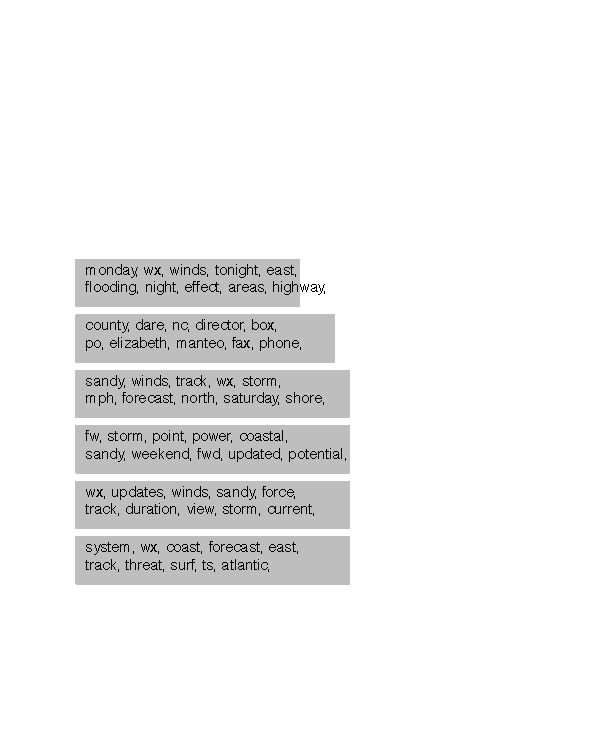
\includegraphics[width = 0.27\textwidth]{images/Output_Dare_internal_clust_topics2.pdf} &
	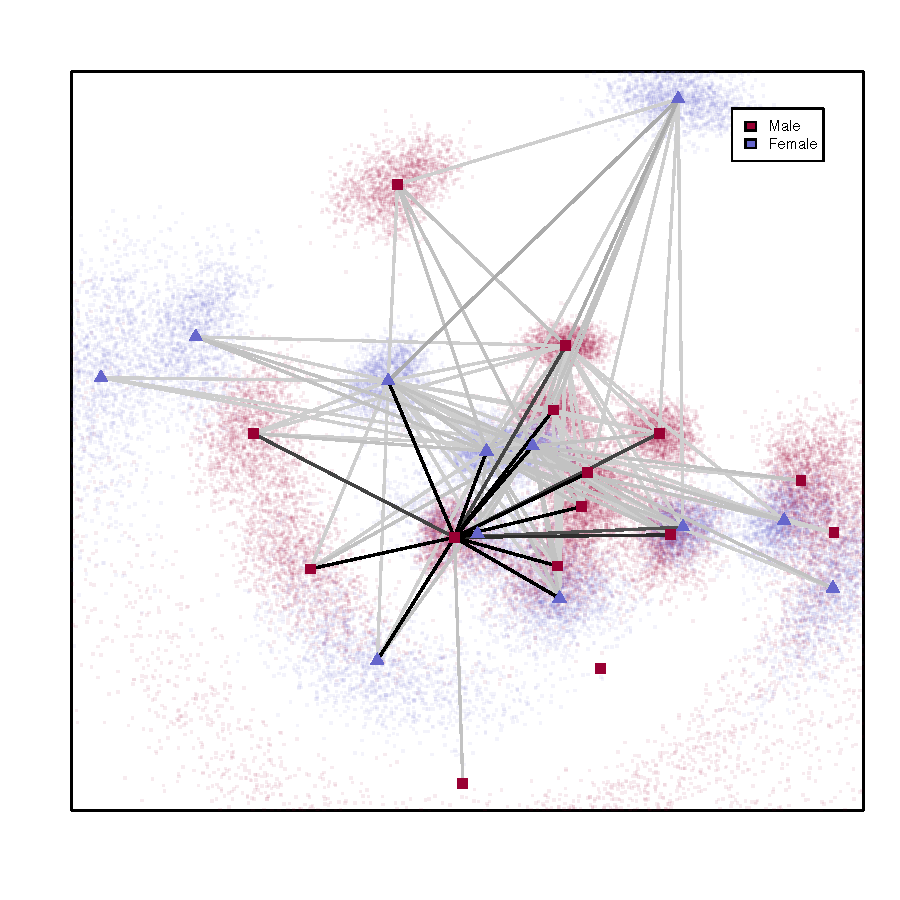
\includegraphics[width = 0.35\textwidth]{images/Output_Dare_internal_Network2.pdf} &
	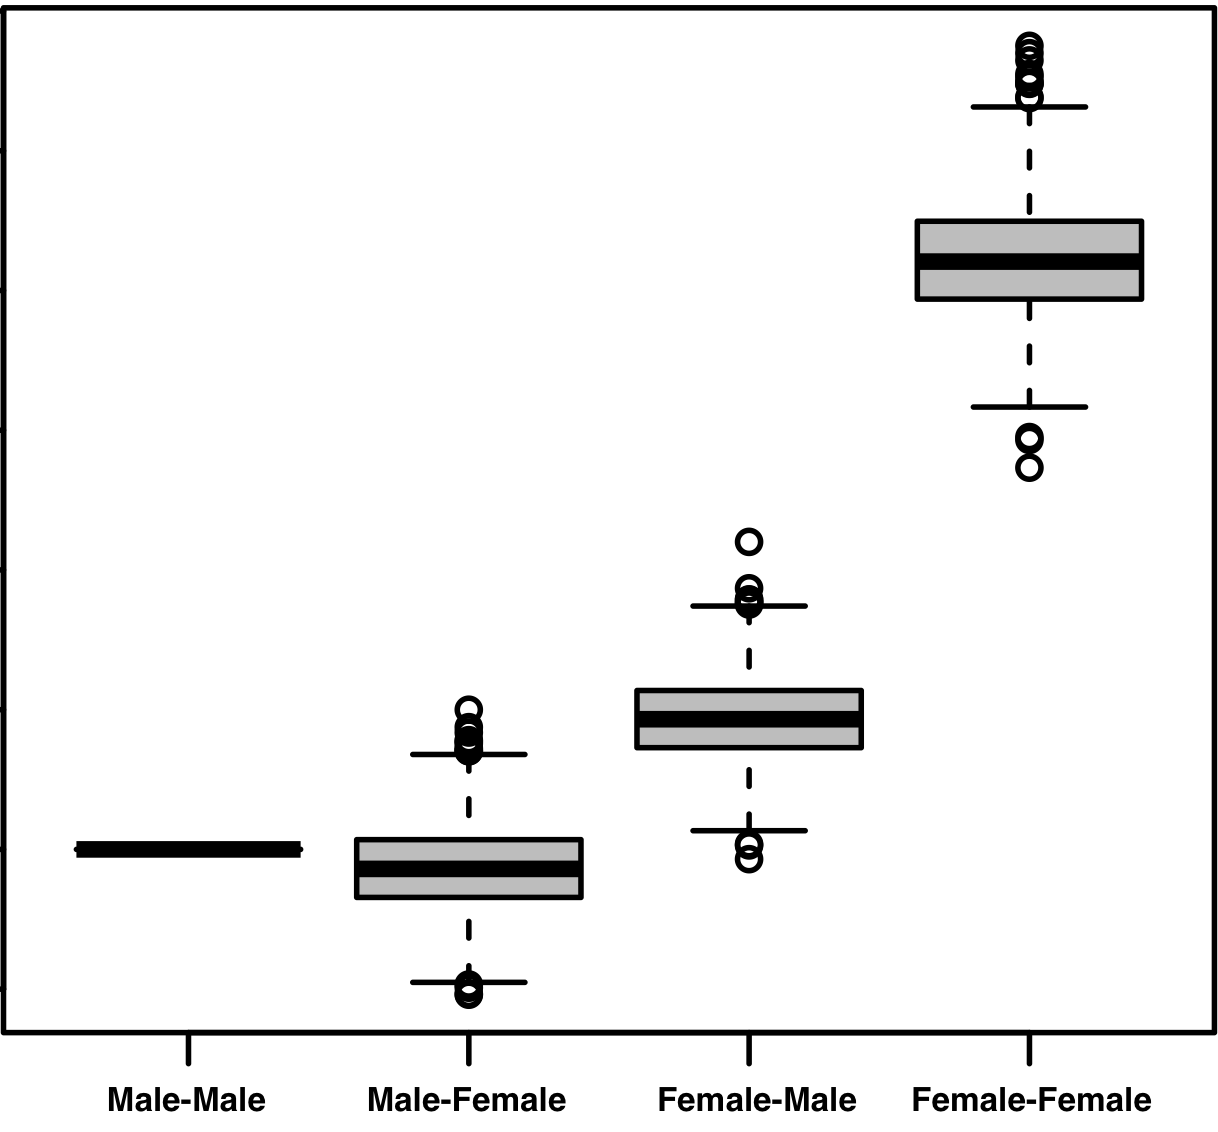
\includegraphics[width = 0.35\textwidth]{images/Dare_Betas_2.png}
	\end{tabular}
	
	\caption{\label{fig:dare results} Model output for selected topic cluster from Dare county. The left-most figure represents the 10 most likely words in the 5 most likely topics (with the most likely topic at the bottom). The middle plot provides latent position estimates for all managers in this county, with female managers represented by blue triangles, and male managers represented by red squares. Point clouds represent 100\% credible intervals for latent position estimates, and the darkness of the edge represents its weight. The box plot on the right depicts mixing parameter estimates.}
	
\end{figure*}


Figure \ref{fig:mixing parameters size} plots the number of managers in a county government (x-axis) against a particular mixing parameter estimate (male-female and female-male) for each of the 4 clusters associated with each of the 17 counties in our sample. Each parameter estimate (dot) is sized by the amount of edge weight assigned to it, to highlight the contribution of more frequent communication patterns. Plots also include LOWESS curves with 95\% confidence bounds. We find that heterophilous communication (male-female and female-male) among department managers tends to be most pronounced in mid-sized county governments in our sample. One potential explanation for this finding is that in small organizations, there may not be a great deal of cross-gender communication because the low number of female managers (in absolute terms) encourages group-cohesion among the minority female managers. Additionally, when the organization is large, the increased access (in absolute terms) to communication partners of the same gender could support a gender-homophily explanation for both male and female managers communication patterns.

\begin{figure}[h]
	\begin{tabular}{cc}
	\textbf{M-F Mixing Parameter} & \textbf{F-M Mixing Parameter}  \\
	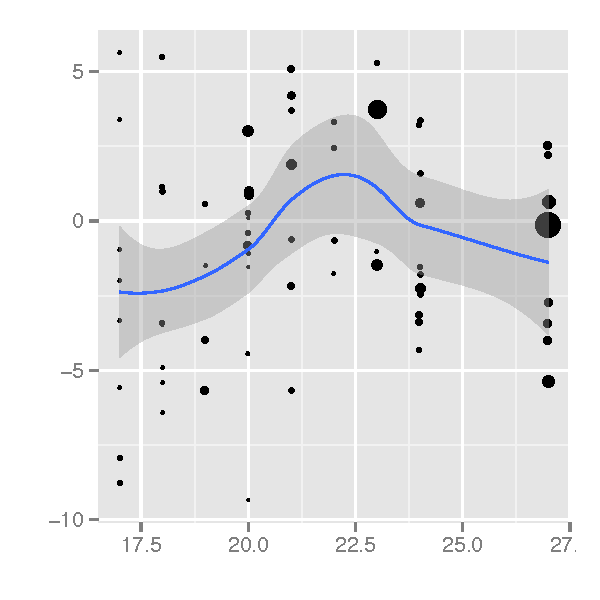
\includegraphics[width = 0.22\textwidth]{images/MF_Size.pdf} &
	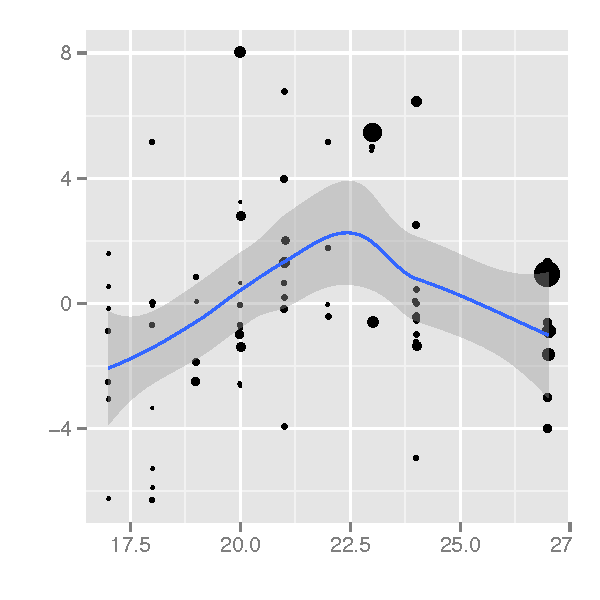
\includegraphics[width = 0.22\textwidth]{images/FM_Size.pdf} \\
	\caption{\label{fig:mixing parameters size} Gender Mixing parameters plotted against the number of department managers, for each of four topic clusters associated with each county.}
	\end{tabular}
	
\end{figure}



%
%

% 	\bigskip
%
% While the analyses presented here are still preliminary, we believe they are beginning to yield insights into the gendering of communication within local governments. These analyses are made possible by the large scale, cross-organization data collection efforts we have undertaken, and we plan to make these data available for other researchers to examine in the future.
\section{Discussion}



\begin{acknowledgments}
This work was supported by US National Science Foundation Grant CISE-1320219 (Hanna Wallach and Bruce A. Desmarais, PIs)
\vspace{-.5cm}
\end{acknowledgments}
\bibliographystyle{plain}
\bibliography{PINLab.bib}


\end{article}



\end{document}


